% Chapter 3

\chapter{Results} % Main chapter title

\label{Results} % For referencing the chapter elsewhere, use \ref{Chapter1} 

\lhead{Chapter 6. \emph{Results}} % This is for the header on each page - perhaps a shortened title

\section{Results}

Figure~\ref{fig:indRunsAvgSize10Fitness} shows $10$ indipendent runs for fitness based search, alongside the mean of these runs' fitness. Following the objective function's gradient fitness based evolution does small step towards better and more optimized individuals from generation to generation. What is more, fitness based evolution often sticks on shapes which then tries to optimize leading the evolution to stop at that local maximum.

\begin{figure}[h!]
\centering
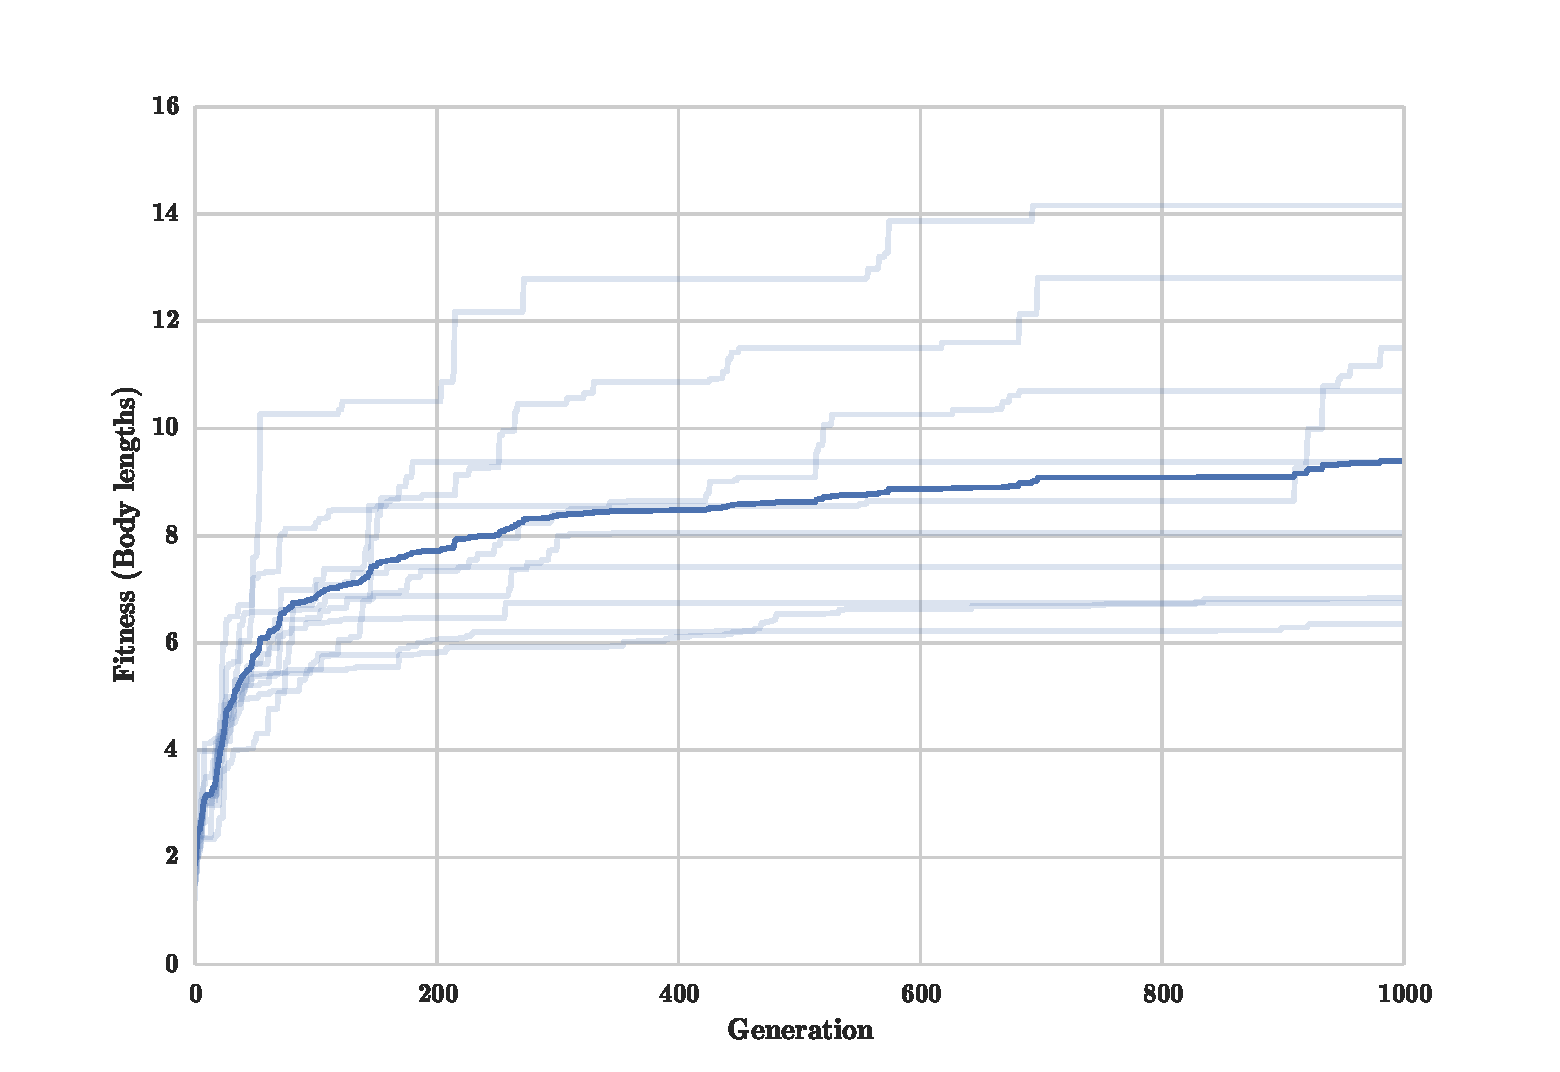
\includegraphics[width=1.0\textwidth]{../Figures/Results/indRunsAvgSize10Fitness.pdf}
\caption{Best fitness so far, average fitness from $10$ individual runs for fitness based search (see \ref{Settings2}).}
\label{fig:indRunsAvgSize10Fitness}
\end{figure}

Figure~\ref{fig:indRunnAvgSize10Novelty} shows $10$ indipendent runs for novelty based search, alongside the mean of these runs' fitness. In comparison with the same figure for fitness based search we can see a clear difference. Evolving for novelty means that within the evolution only a novel behavior is rewarded instead of a good behavior or a behavior that leads to the optimization of the objective function. Big steps in the fitness value on all independent runs can be observed which can lead us to a conclusion that there is no such a function as optimization of current good individuals within the evolution process. Initially novel individuals are highly rewarded, these individuals could be very good in respect to the fitness or not, the algorithm does not consider how individuals can be measured in respect to the objective function and does not have any information regarding this either. On the next generation, mutations, crossovers, or even copies of these novel individuals are not going to be highly variant in respect to their genotype's topology from their ancestors, resulting to similar behaviors which are going to be unremarkably rewarded as far as their novelty is concerned. Thus, highly novel individuals are producing less novel children, meaning that these children, even though their fitness is high, will not have the chance to reproduce in the next generations and be improved eventually, as in fitness based evolution..

\begin{figure}[h!]
\centering
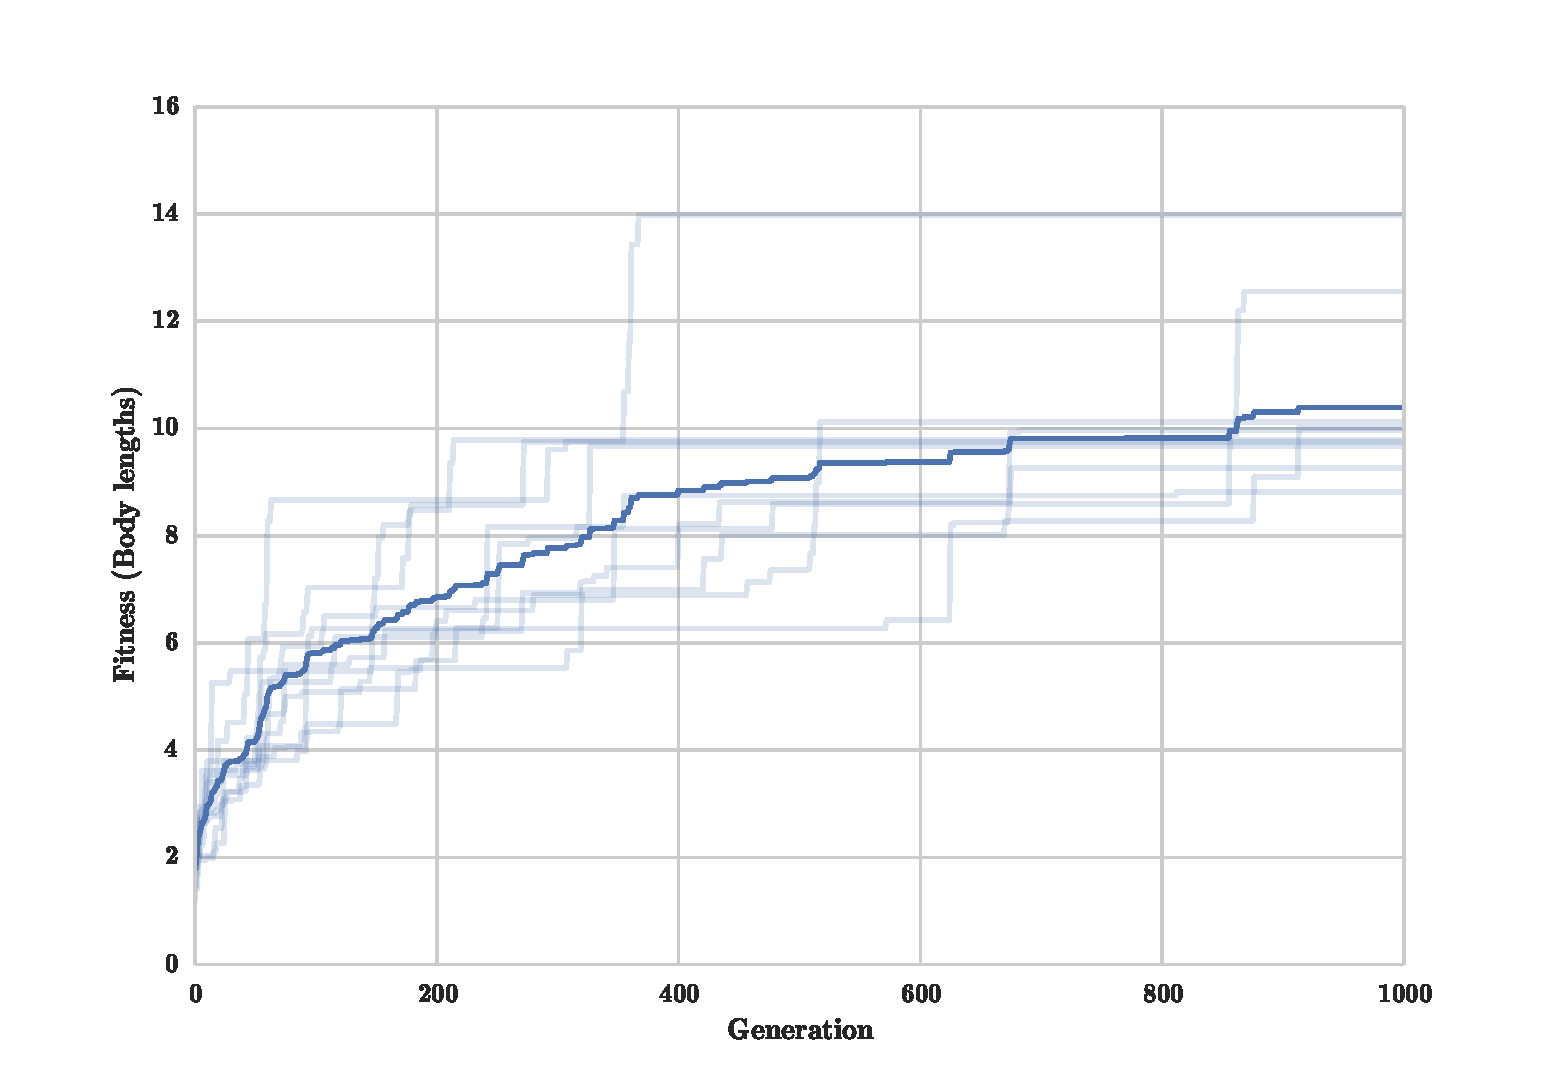
\includegraphics[width=1.0\textwidth]{../Figures/Results/indRunnAvgSize10Novelty.pdf}
\caption{Best fitness so far, average fitness from $10$ individual runs for novelty search (see \ref{Settings2}).}
\label{fig:indRunnAvgSize10Novelty}
\end{figure}


\begin{figure}
\centering
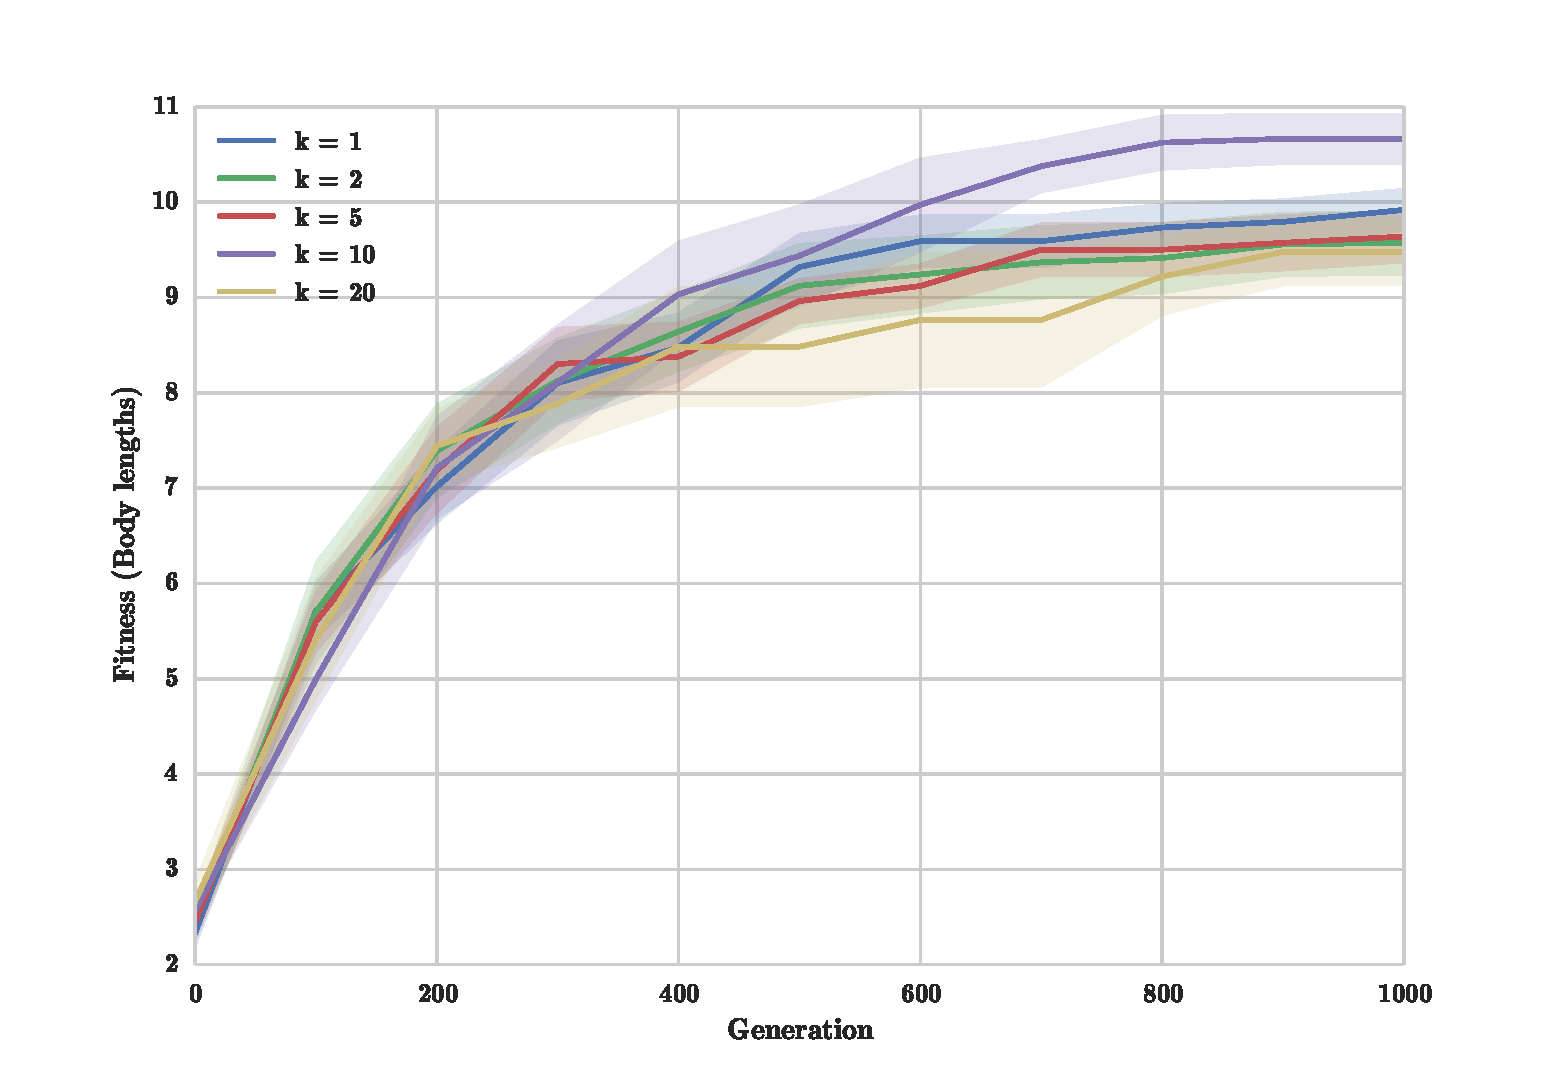
\includegraphics[width=1.0\textwidth]{../Figures/Results/KnnExperimentSize5.pdf}
\caption{Best so far fitness averaged over $10$ runs (see \ref{Settings1}), for different $k$ to sparsity computation of the behavior.}
\label{fig:KnnExperimentSize5}
\end{figure}

\begin{figure}[h!]
\centering
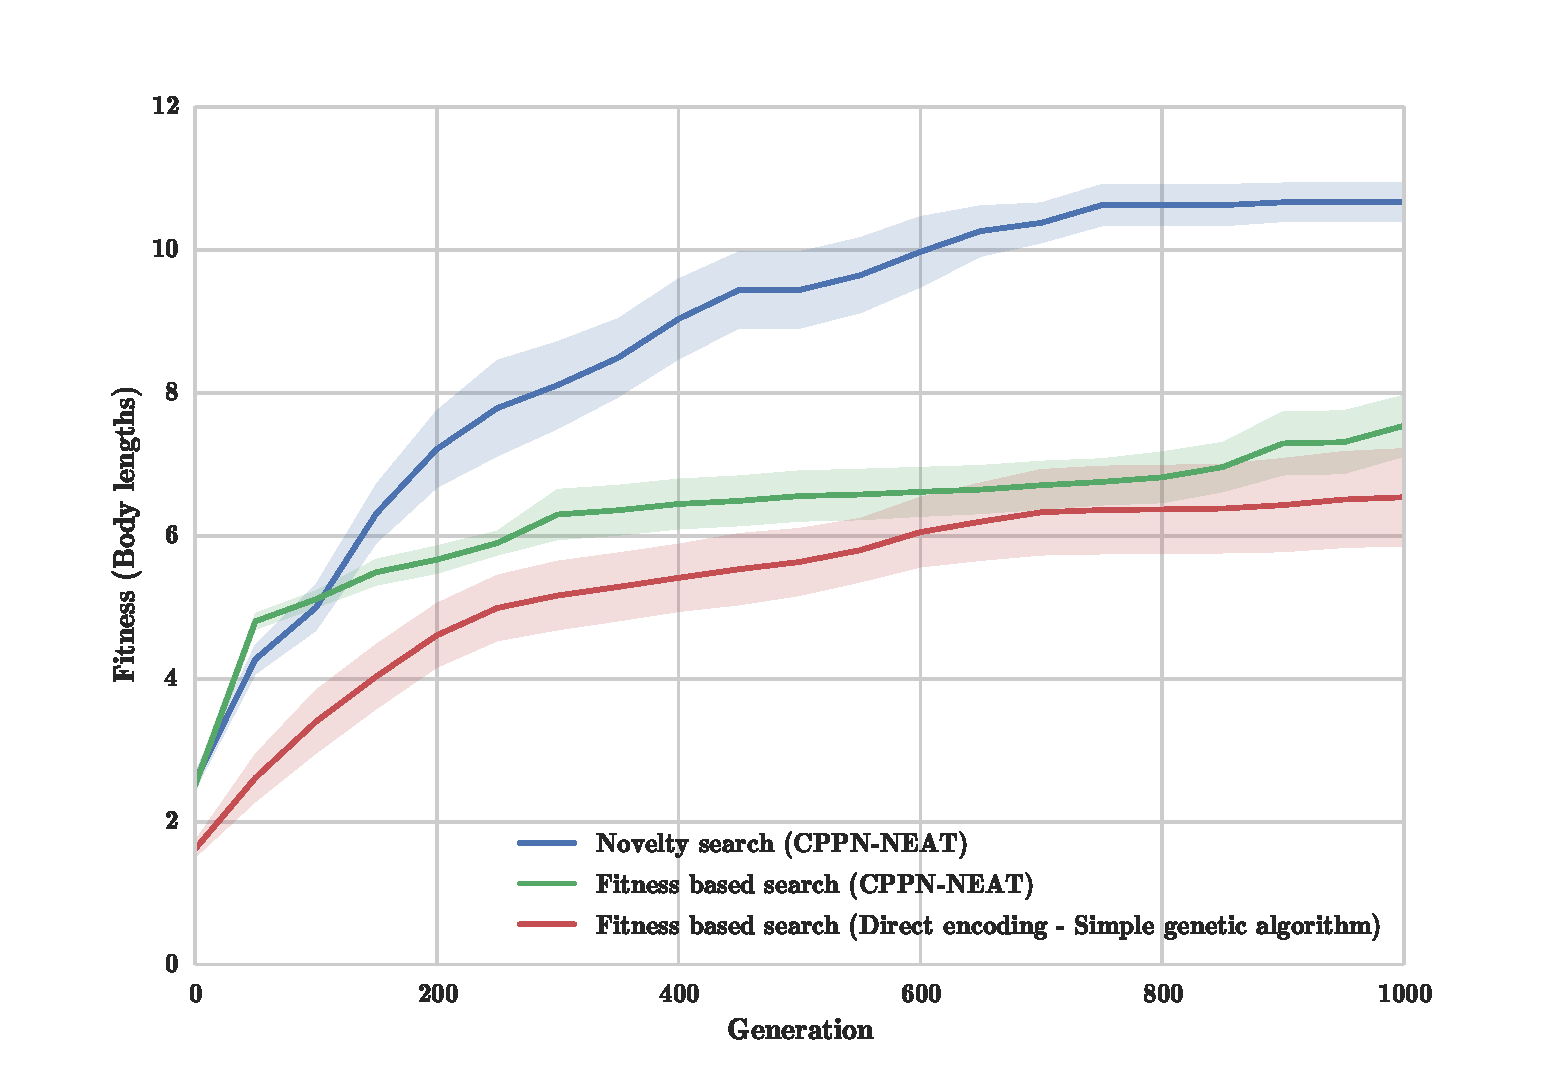
\includegraphics[width=1.0\textwidth]{../Figures/Results/FitvsNovVsDirSize5.pdf}
\caption{Comparison of simple genetic algorithm (direct encoding) against \emph{fitness} - \emph{novelty} search with generative encoding. Best so far fitness averaged over $10$ runs (see \ref{Settings1}).}
\label{fig:FitvsNovVsDirSize5}
\end{figure}


\begin{figure}[h!]
\centering
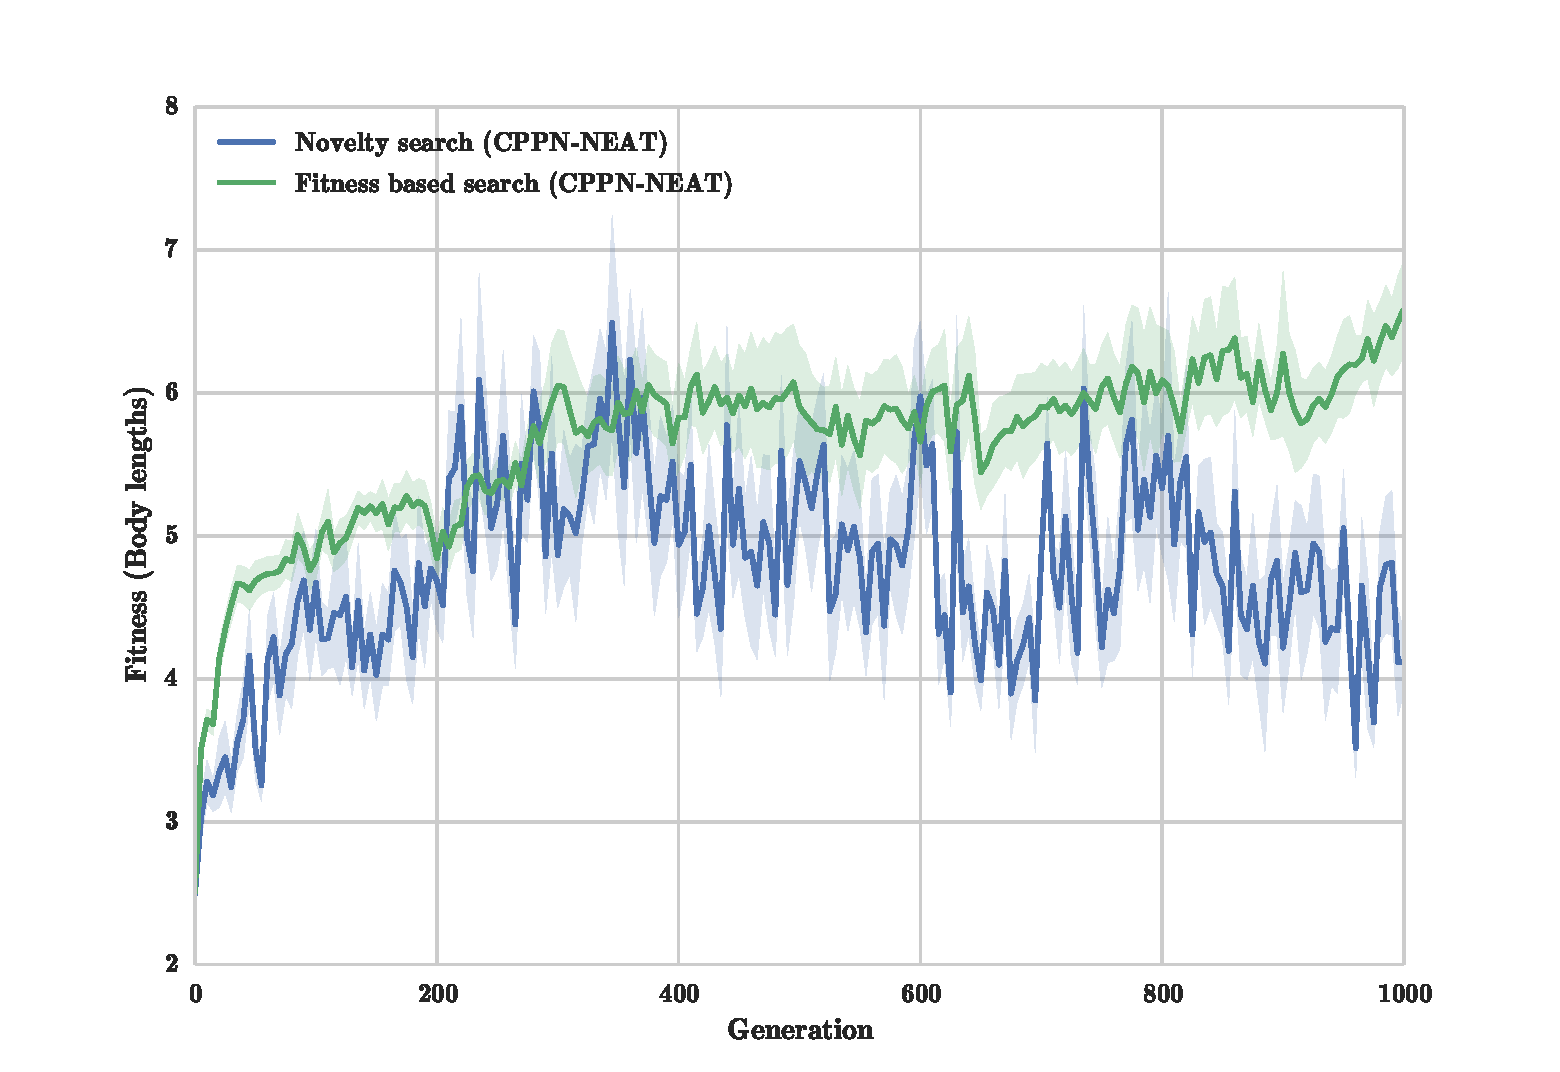
\includegraphics[width=1.0\textwidth]{../Figures/Results/AvgGenerChampNoveltyFitnessSize5.pdf}
\caption{Fitness of the generation's champion (best individual) for \emph{fitness} - \emph{novelty} search averaged over $10$ runs (see \ref{Settings1}).}
\label{fig:AvgGenerChampNoveltyFitnessSize5}
\end{figure}

\begin{figure}[h!]
\centering
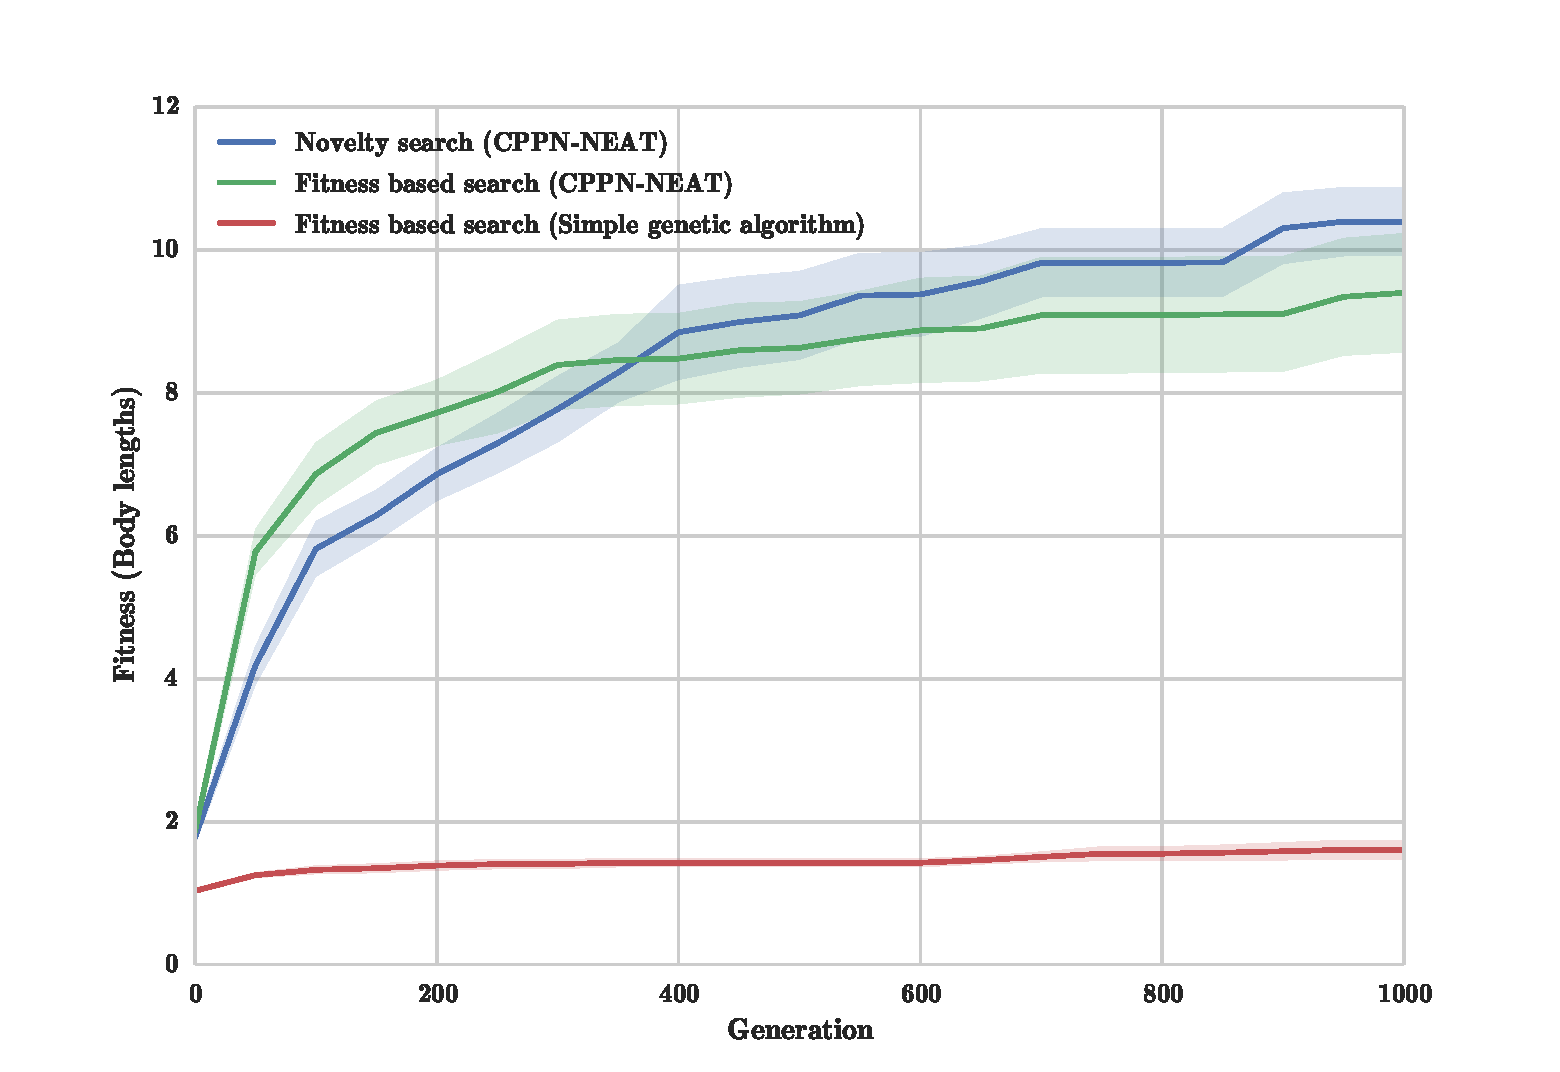
\includegraphics[width=1.0\textwidth]{../Figures/Results/FitvsNovVsDirSize10.pdf}
\caption{Comparison of simple genetic algorithm (direct encoding) against \emph{fitness} - \emph{novelty} search with generative encoding. Best so far fitness averaged over $10$ runs (see \ref{Settings2}).}
\label{fig:FitvsNovVsDirSize10}
\end{figure}

\begin{figure}
\centering
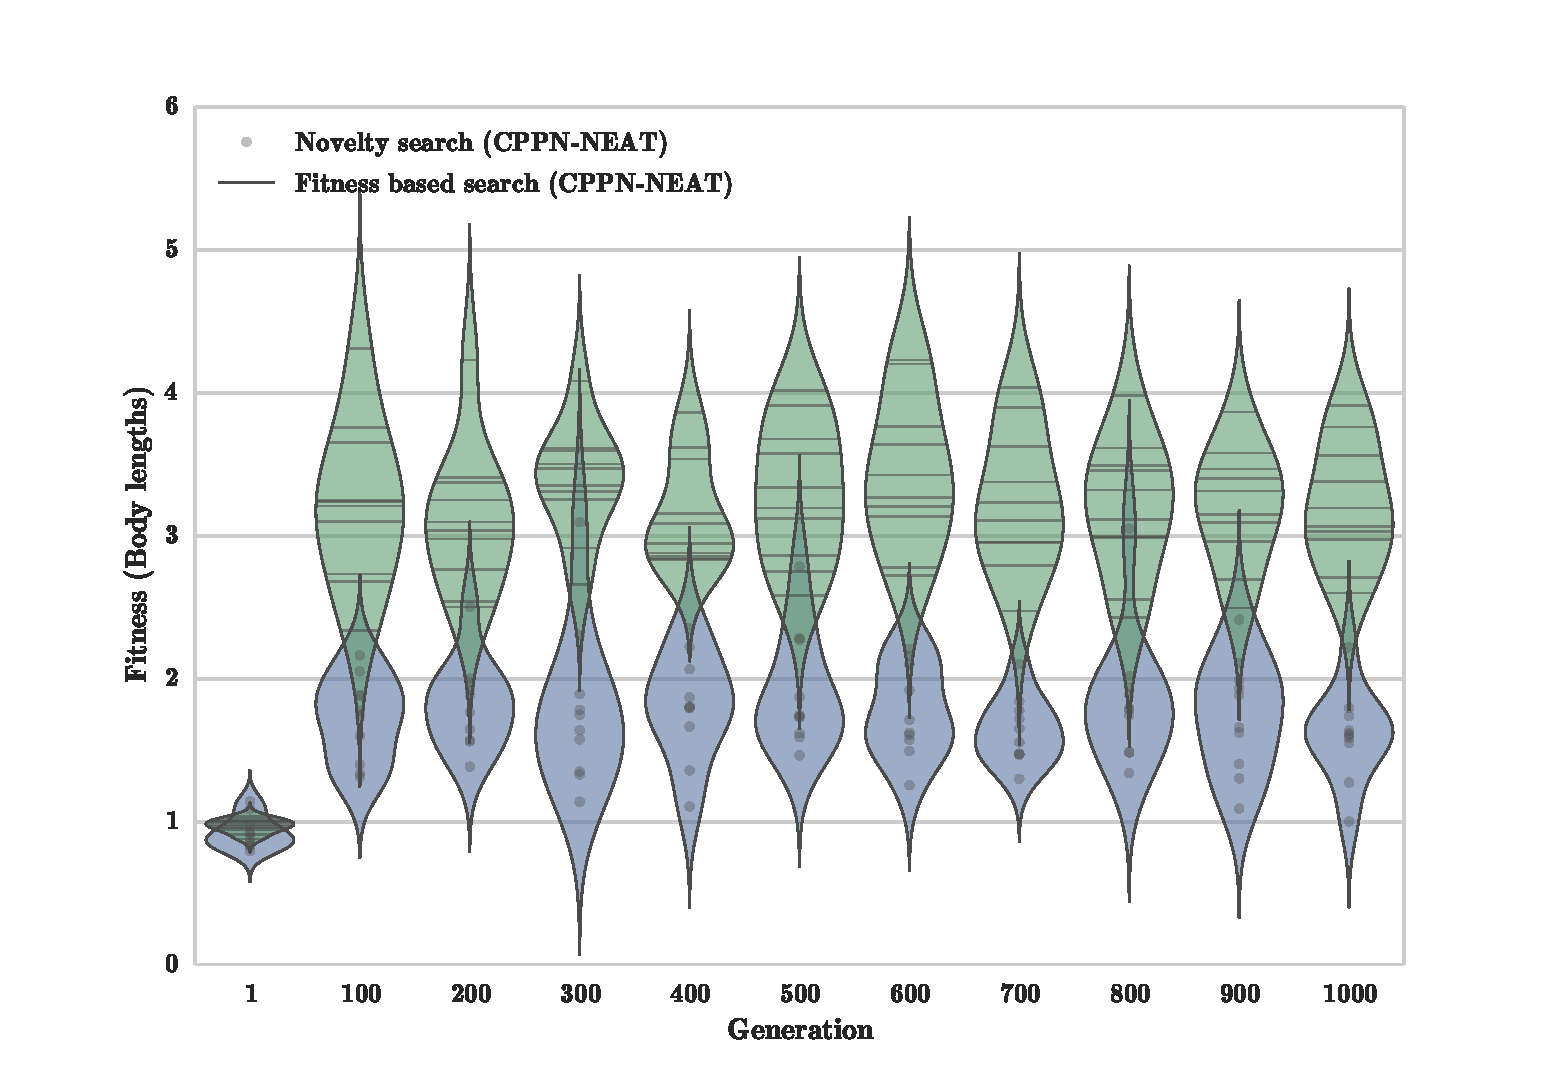
\includegraphics[width=1.0\textwidth]{../Figures/Results/ViolinPlotsAvgGenFitSize5.pdf}
\caption{Distributions of average population fitness per generation over 10 runs for \emph{fitness}(green) - \emph{novelty} (blue) search with generative encoding (see \ref{Settings2}).}
\label{fig:ViolinPlotsAvgGenFitSize5}
\end{figure}


\begin{figure}
\centering
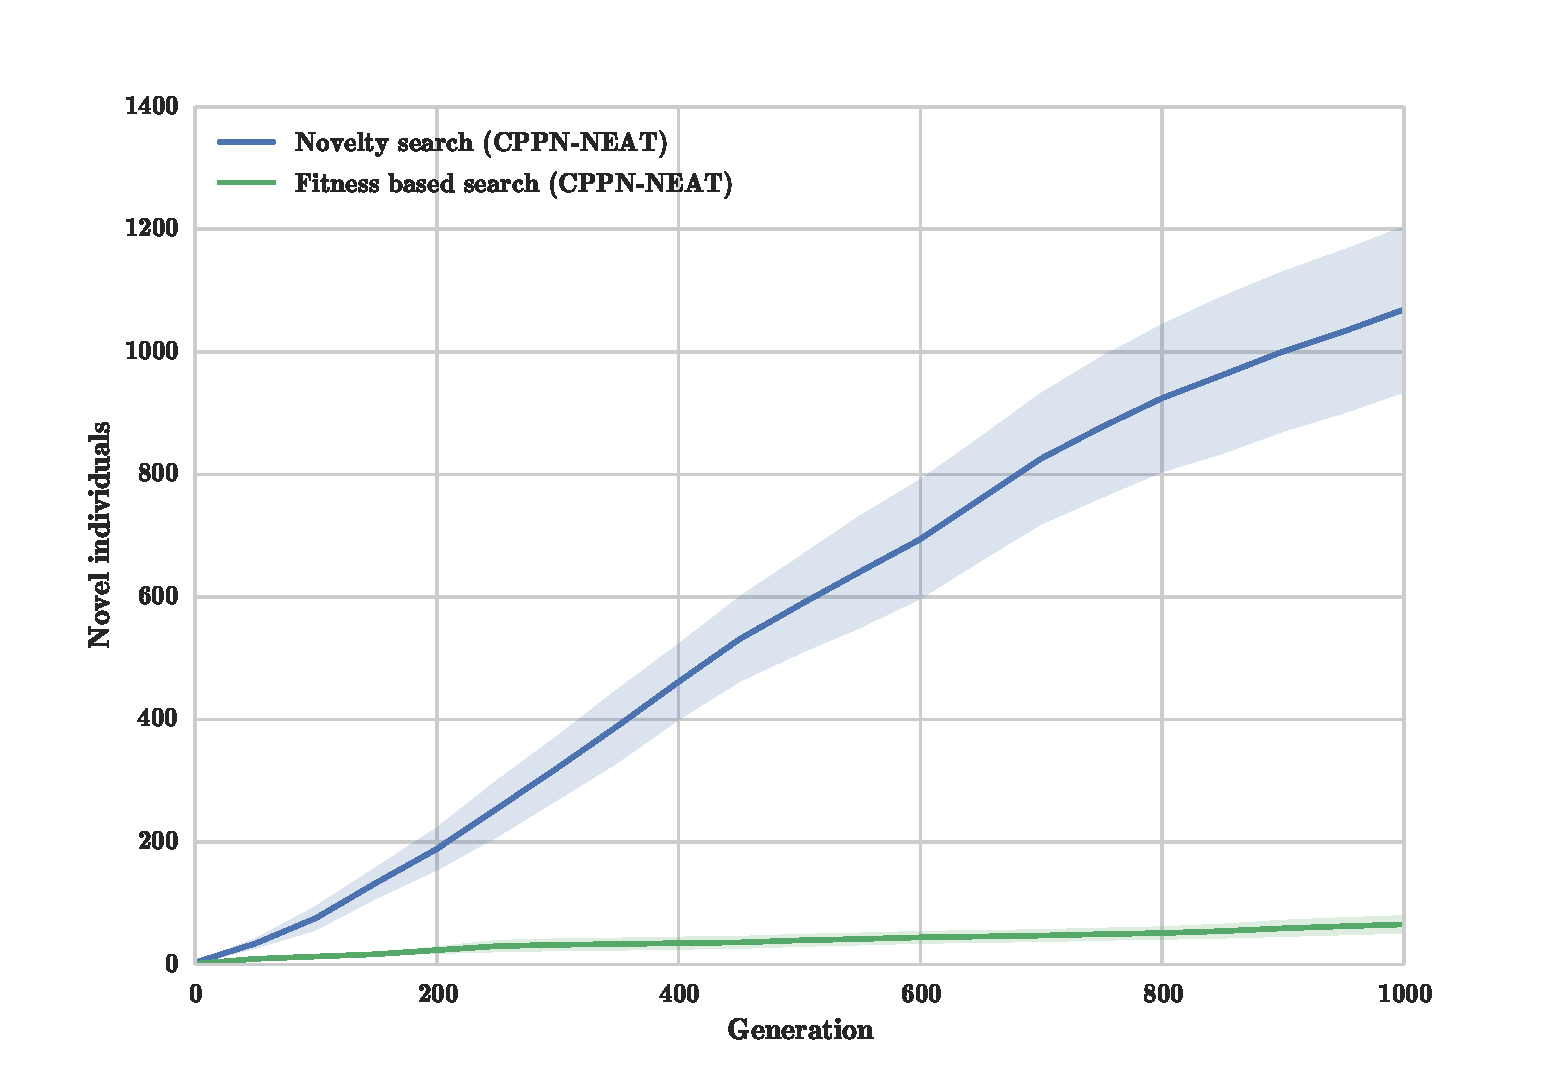
\includegraphics[width=1.0\textwidth]{../Figures/Results/novelIndividualsFitNovComp.pdf}
\caption{Number of novel behaviors up to generation number, averaged over 10 runs. The novelty measure is computed as the average distance from the $10$-nearest behaviors for \emph{fitness} - \emph{novelty} search with generative encoding (see \ref{Settings1}).}
\label{fig:novelIndividualsFitNovComp}
\end{figure}


\begin{figure}
\centering
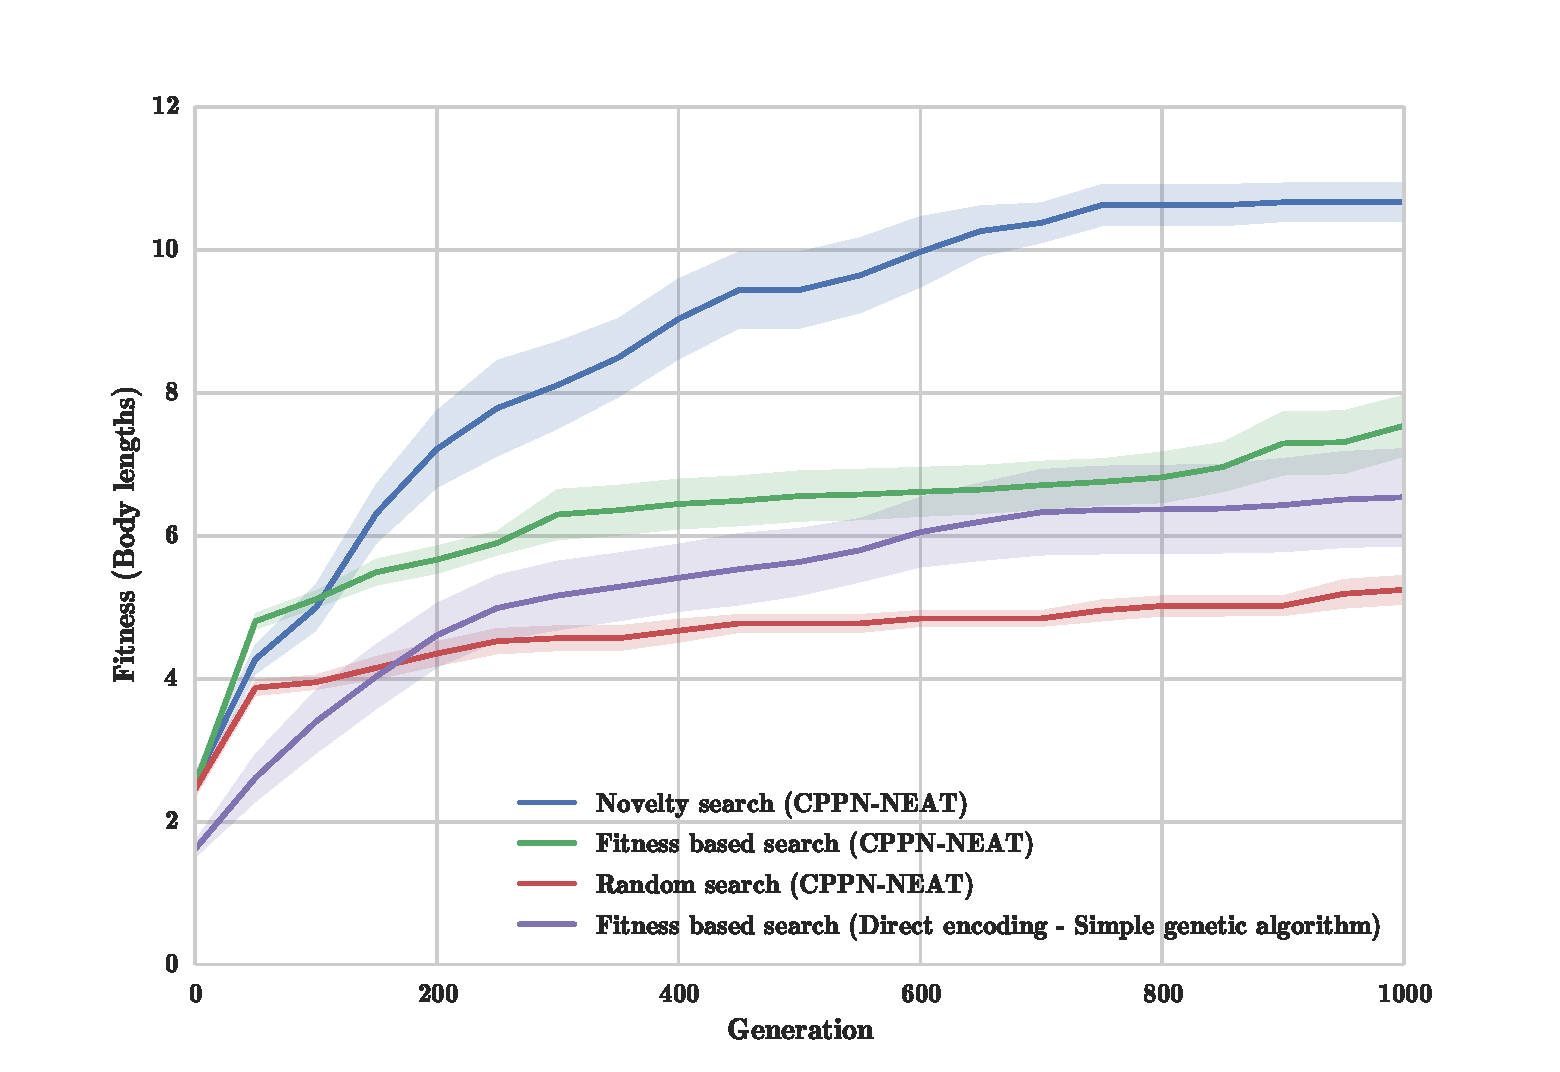
\includegraphics[width=1.0\textwidth]{../Figures/Results/FitNovRandomDirectSize5.pdf}
\caption{Comparison of simple genetic algorithm (direct encoding) against \emph{random} - \emph{fitness} - \emph{novelty} search with generative encoding. Best so far fitness averaged over $10$ runs (see \ref{Settings1}).}
\label{fig:FitNovRandomDirectSize5}
\end{figure}

\begin{figure}
\centering
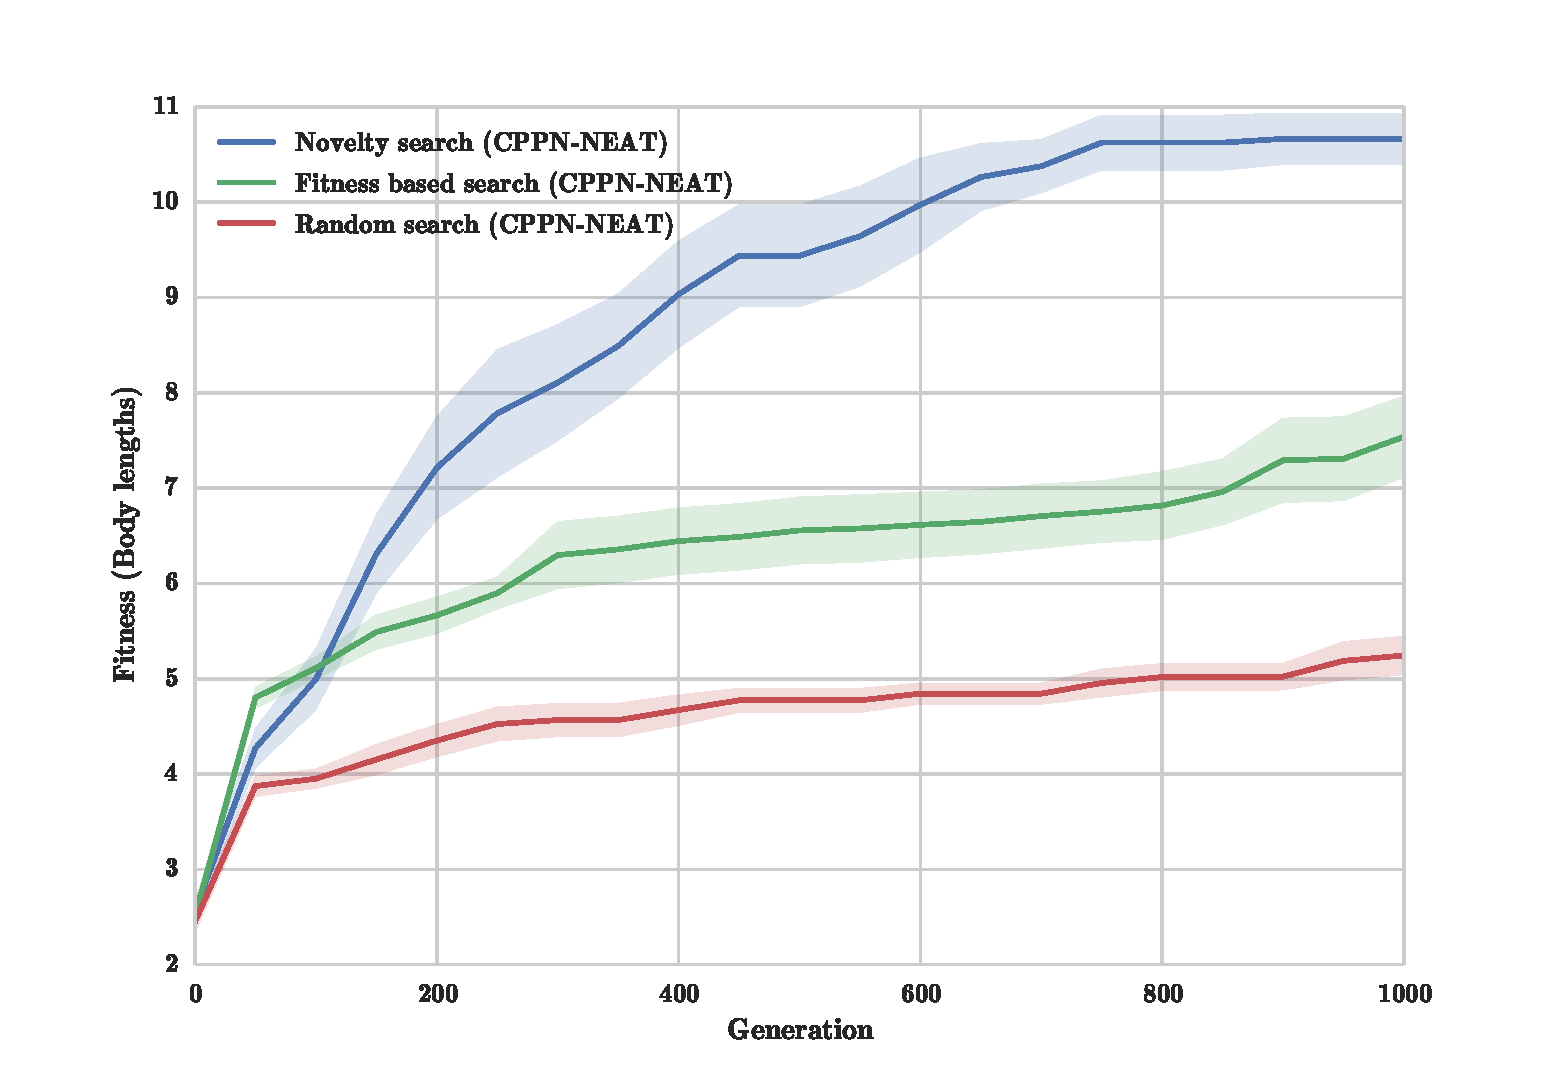
\includegraphics[width=1.0\textwidth]{../Figures/Results/FitNovRandomSize5.pdf}
\caption{Comparison of \emph{random} - \emph{fitness} - \emph{novelty} search with generative encoding. Best so far fitness averaged over $10$ runs (see \ref{Settings1}).}
\label{fig:FitNovRandomSize5}
\end{figure}


\begin{figure}
\centering
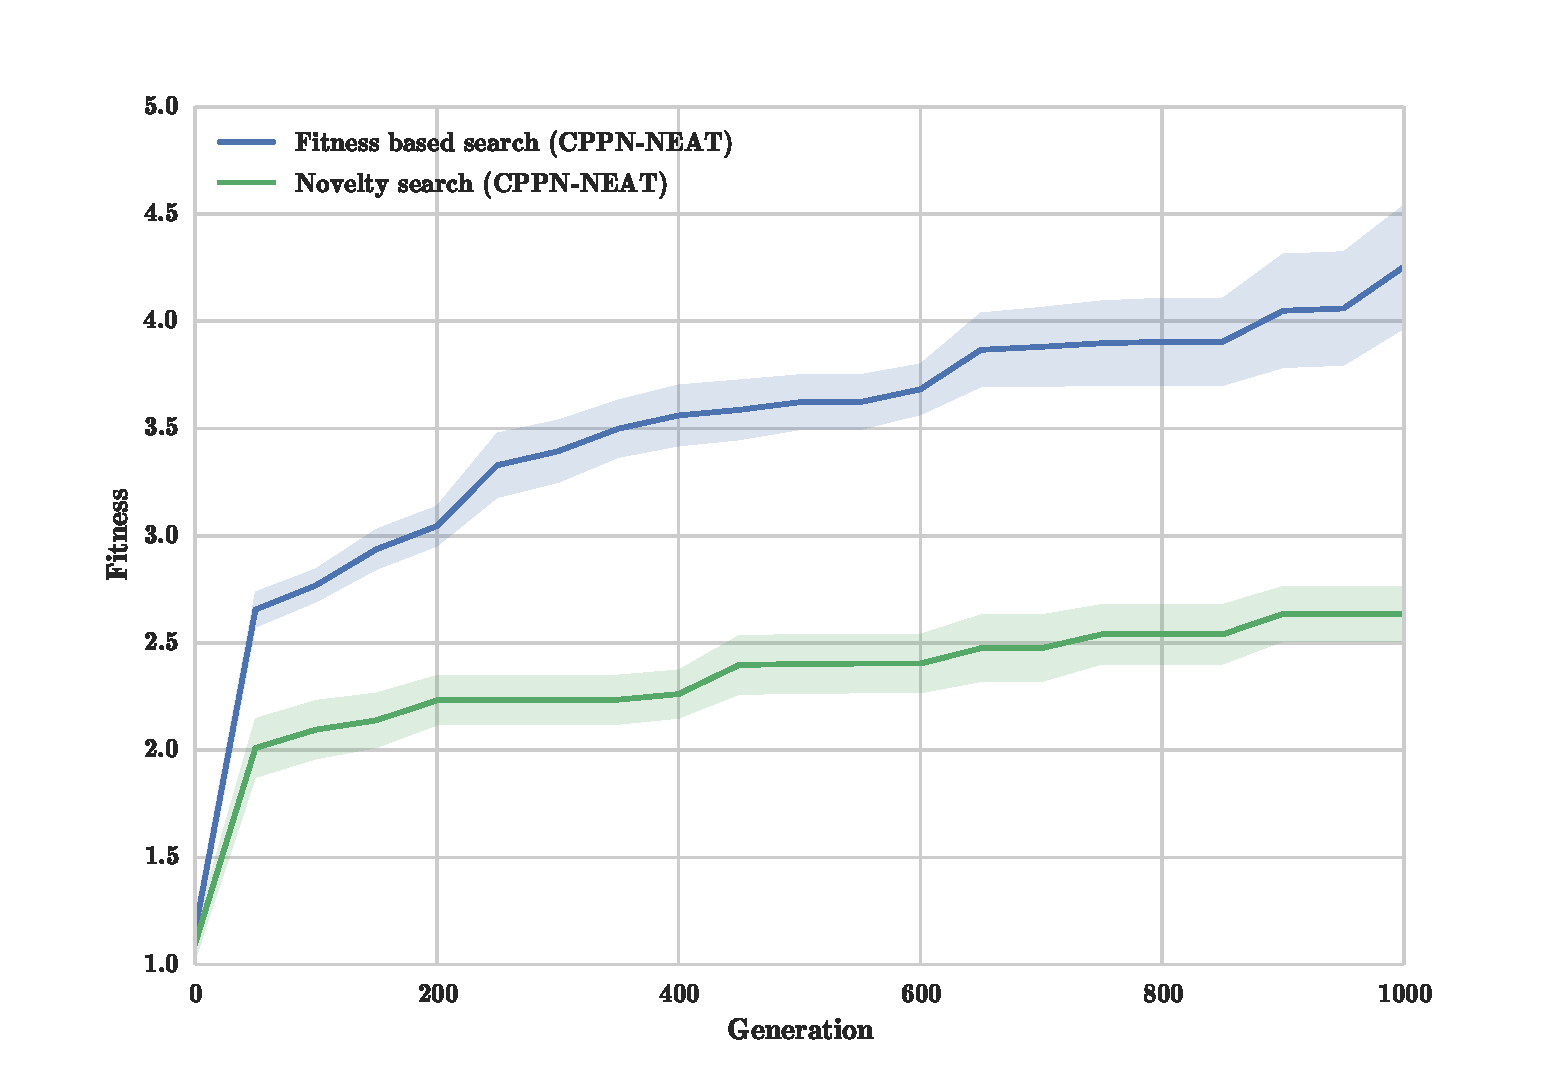
\includegraphics[width=1.0\textwidth]{../Figures/Results/FitNovSize5Pen2.pdf}
\caption[]{Best so far fitness averaged over $10$ runs, penalizing actuated materials\footnotemark for \emph{fitness} - \emph{novelty} search with generative encoding (see \ref{Settings1}).}
\label{fig:FitNovRandomSize5}
\end{figure}

\footnotetext{Actuated materials penalize fitness: \[f = (1 - (n_{actuated} / n_{total})^{1.5}) \times disp \], where $n_{actuated}$, is the number of actuated voxels, $n_{total}$ total number of voxels and $disp$ the displacement of the softbot's center of mass.}

\begin{figure}[h!]
\centering
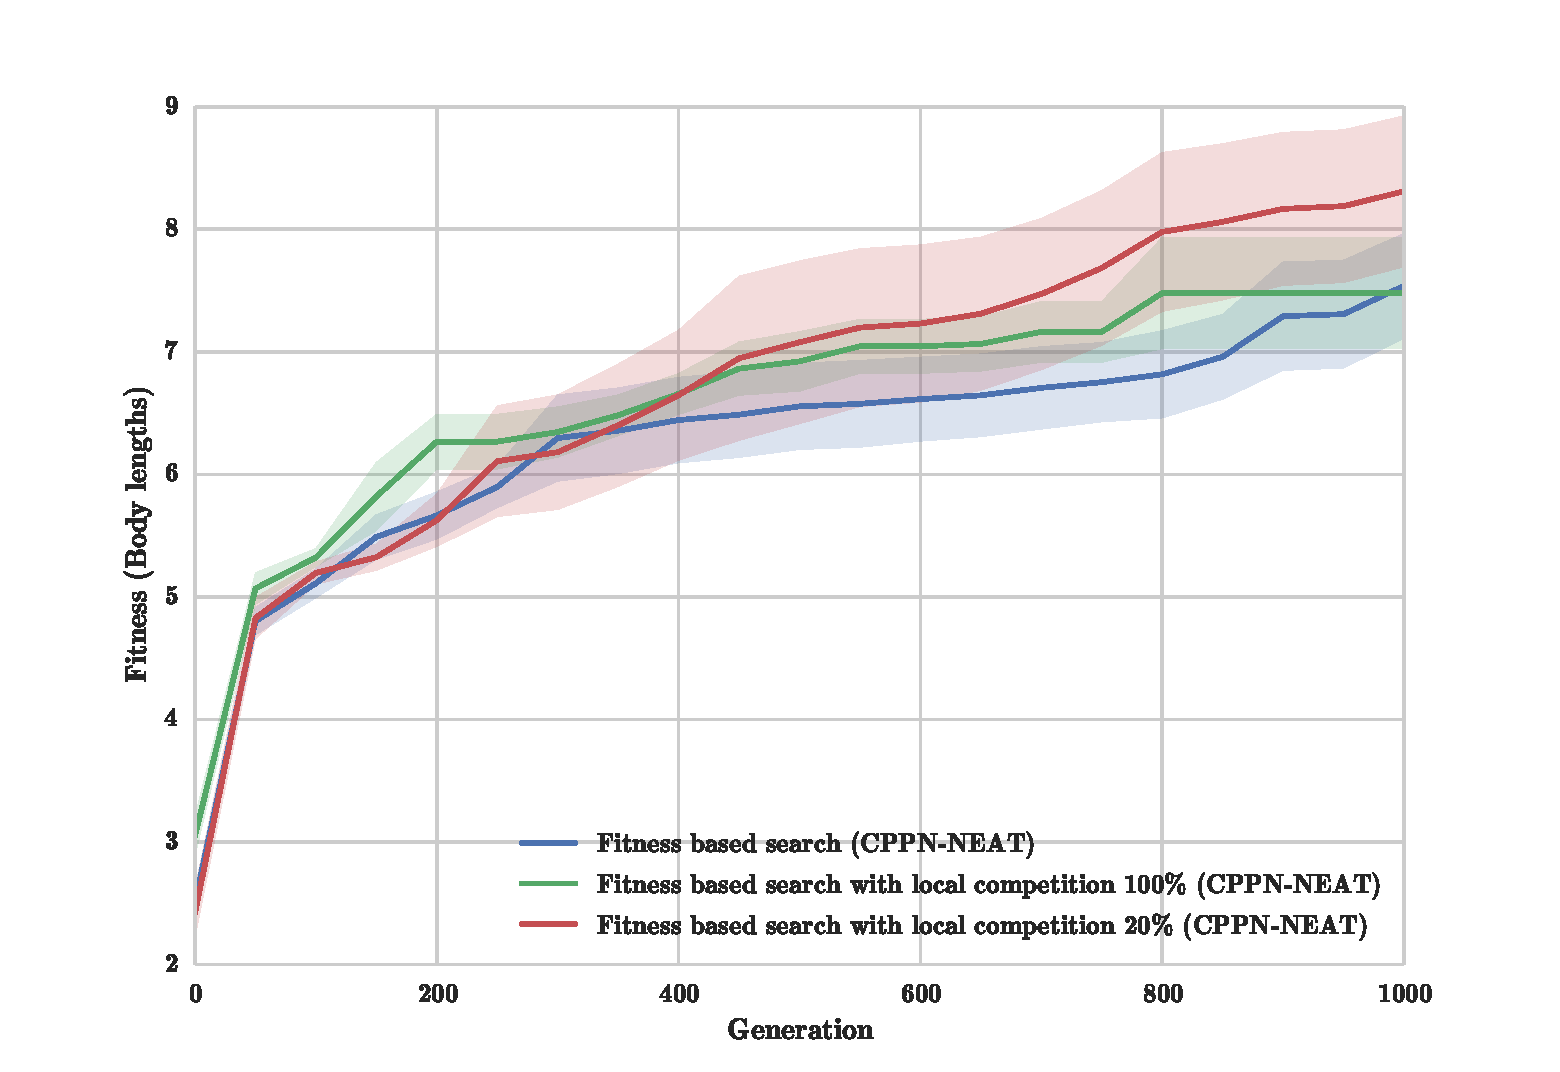
\includegraphics[width=1.0\textwidth]{../Figures/Results/fitComp100_20percent.pdf}
\caption{Best so far fitness averaged over $10$ runs, with no competition, local competition among the top $20\%$ and in the complete population of each species for \emph{fitness} search (see \ref{Settings1}).}
\label{fig:fitComp100_20percent}
\end{figure}

\begin{figure}[h!]
\centering
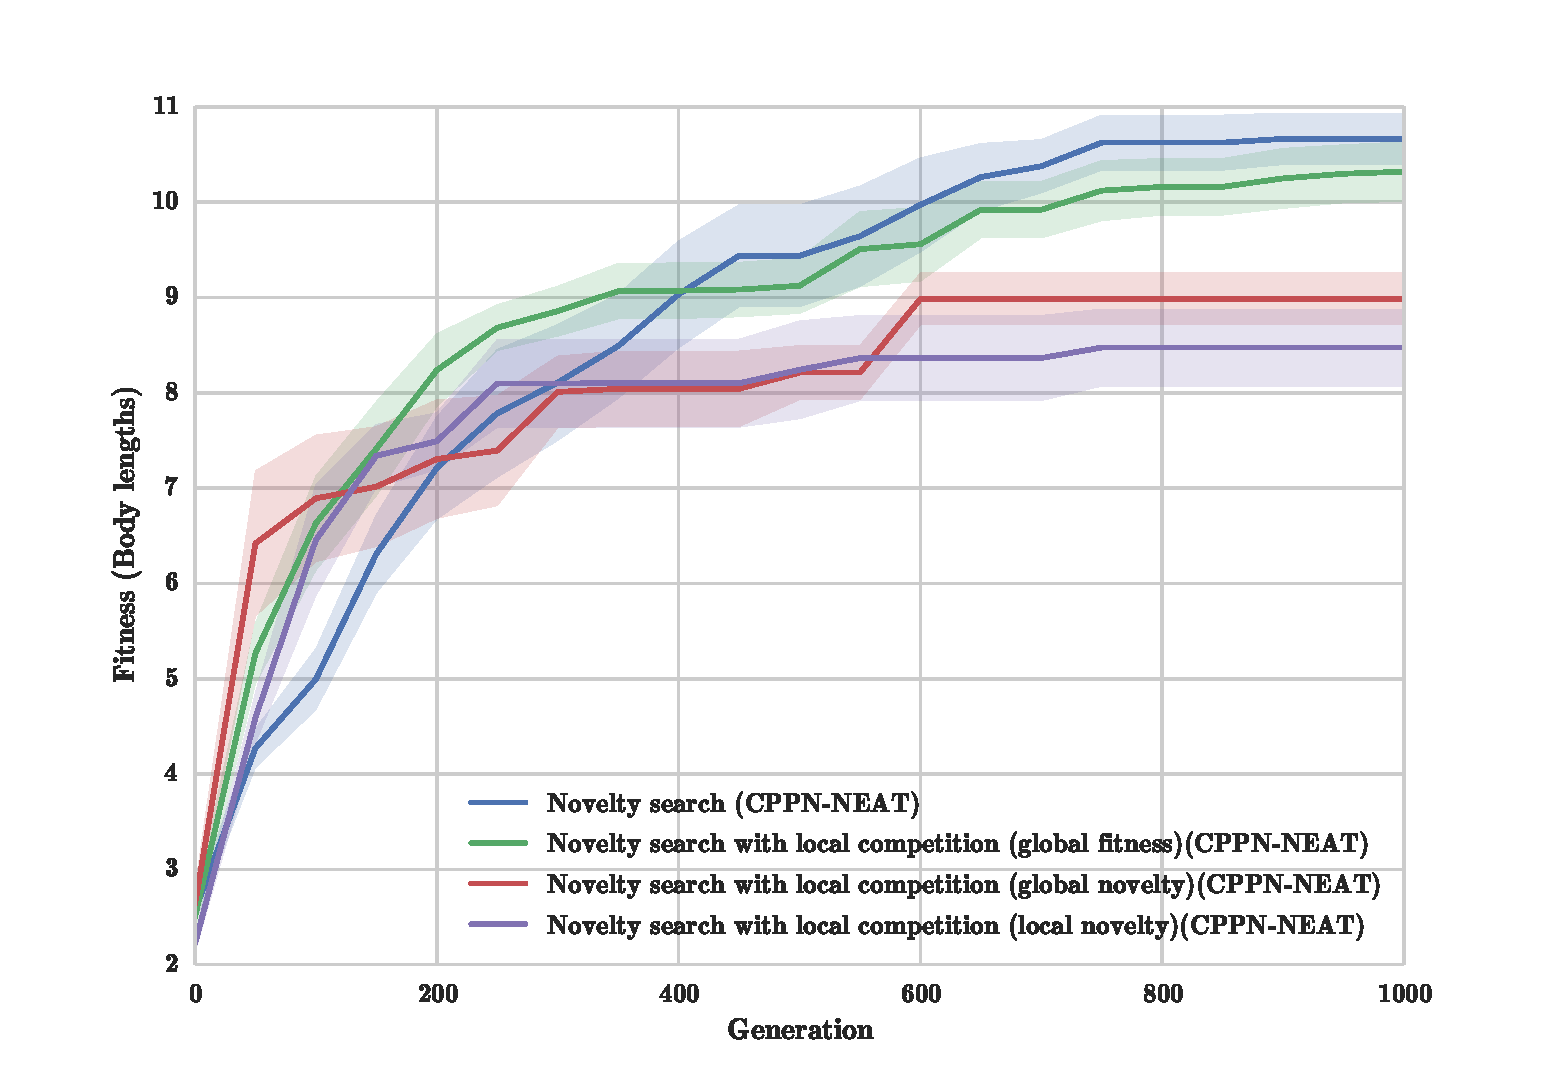
\includegraphics[width=1.0\textwidth]{../Figures/Results/NoveltyCompetitionsSize5.pdf}
\caption{Best so far fitness averaged over $10$ runs, for local competition held among the population of each species for \emph{novelty} search with generative encoding (see~\ref{Settings1}).}
\label{fig:NoveltyCompetitionsSize5}
\end{figure}


\begin{figure}[h!]
\centering
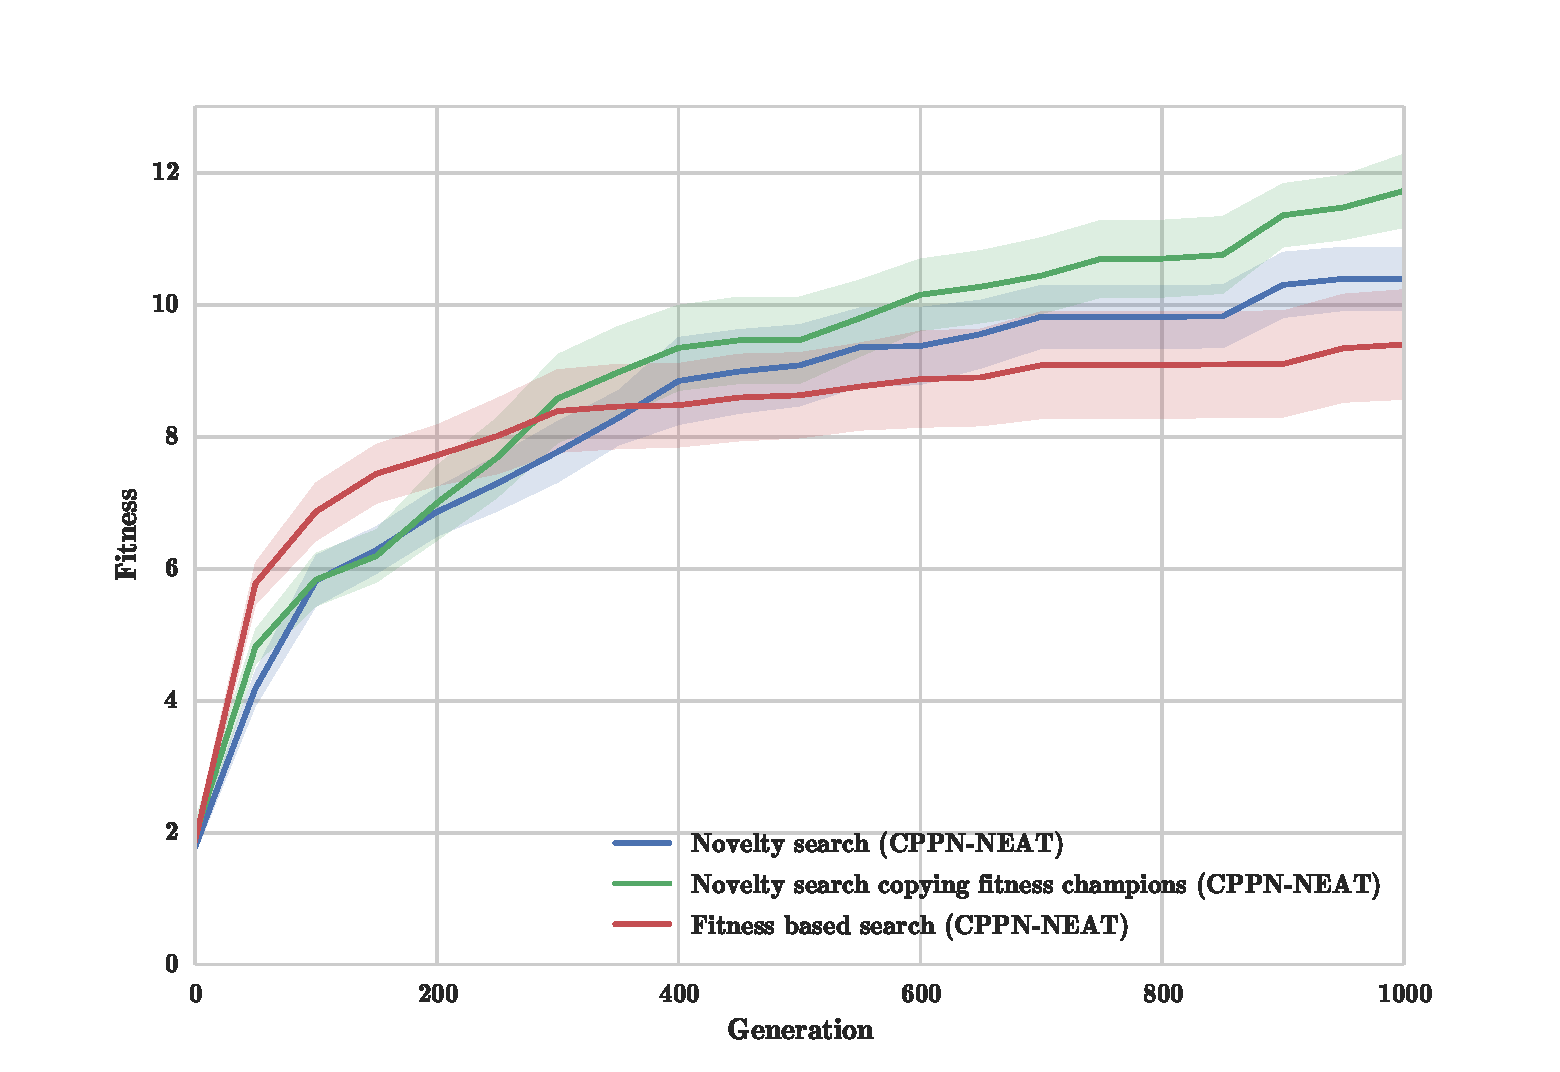
\includegraphics[width=1.0\textwidth]{../Figures/Results/CopyFitChampions10.pdf}
\caption{Best so far fitness averaged over $10$ runs, for \emph{novelty} search with and without copying \emph{fitness} champions within species  with generative encoding (see~\ref{Settings1}).}
\label{fig:CopyFitChampions10}
\end{figure}

